\section*{Exercise 15}
\addcontentsline{toc}{section}{Exercise 15}
In this exercise I have used the Implementation of MD5 found in java's
java.security.MessageDigest library. Java uses 32bit integers and assumes all
things to be signed, this still leaves plenty of space for our $2^{20}$bit
hashes.\\
To limit the size of the input/output of the funktion I have chosen to AND the
value with a bitmask of 0xfffff, as this truncates any results that are larger.
My implementation of the MD5-redux then looks like this:\\
\begin{lstlisting}
	public static int getMD5Hash(int hexInput, int bitSizeLimiter)
	{
		try
		{
			//calculate the limit to use as a bit-mask
			int mask = (int) (Math.pow(16, (bitSizeLimiter / 4))-1);
			//use the mask to set any bits above the wanted limit to 0.
			hexInput = mask & hexInput;
			
			//get the byte value 			   4 bytes for a 32-bit integer
			byte[] bytes = ByteBuffer.allocate(4).putInt(hexInput).array();
			
			//create a MD5 digest
			MessageDigest md = MessageDigest.getInstance("MD5");
			md.update(bytes);
			byte[] digest = md.digest();

			//get the integer value
			int result = ByteBuffer.wrap(digest).getInt();
			
			//use the mask again to limit the output
			result = mask & result;
			return result;
		}
		catch (Exception e)
		{
			System.err.println(e.getMessage());
			e.printStackTrace();
		}
		return 0;
	}
\end{lstlisting}
Using this I then run the desired $2^{16}$ chains of $2^{8}$ length and count
how many of the possible keys i have reached every 100 chains. The result as
seen in figure~\ref{fig:Hellman} only covers a lacluster $\approx
27\%$ of the key space.
\FloatBarrier
\begin{figure}[h]
\centering
\makebox[\textwidth]{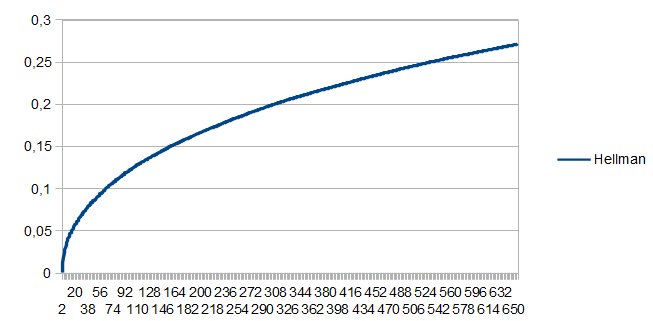
\includegraphics[width=\textwidth]{Hellman}}
\caption{\emph{Coverage}: This model does not even cover a third of the
keyspace}
\label{fig:Hellman}
\end{figure}
\FloatBarrier